\section{Evaluation}
\label{sec:eval}

In this section, we first illustrate the expressivity and reusability of \gaia{} by an animation gallery with a wide range of examples\footnote{Available in supplementary materials}. 
We conducted a user study with non-experts in animation creation, where we focused on observing the ease of use and the learning curve of \gaia{}. 
Finally, we performed semi-structured interviews with the experts who have used \gaia{} in their projects, to further understand the advantages and limitations of \gaia{}.

\subsection{Example Gallery}

\gaia{}'s expressiveness lies in two aspects: the compatibility of different kinds of infographics created by different tools and the capability to efficiently express a variety of complex animations.
Therefore, we built an animation gallery with a wide range of examples including
(1) replications of real-world data videos with different topics and styles; 
(2) generated visualizations created by Vega-Lite; and 
(3) animations of infographics adapted from related work \cite{ge2020canis,wang2021animated, cui2021mixed}.
These examples not only cover a wide range of infographic types, such as isotypes, timelines and different kinds of informative charts but also involve all animation semantic types introduced in \cite{cheng2022investigating}.
Each example includes a top-level animation spec, a set of templates used (some of them are reused from other examples), a static SVG and a corresponding binder that maps the SVG to the target type tree\footnote{For SVGs generated by Vege-Lite, binder specs can be generated automatically because the structure of SVGs is fixed.}.

As a key design goal of \gaia{}, reusability of \gaia{} enables sharing the animation design.
A lot of reuse in our gallery also simplifies the complexity of specs.
For instance, template \code{BarChartEnter} is used in the example \textit{Australia Fire}, \textit{Transportation Mode} and \textit{Wealth Inequality}.
In the example \textit{GDP Comparison} and \textit{2017 DC Courst}, template \code{ShowCategory} are invoked with different parameters, as they all include several similar entering animations for bars, bar labels, and axis labels/symbols.
To further show the reusability, we use templates to create all animations in the examples for Vega-Lite generated charts.
The template \code{ChartFrameworkEnter} is reused across the bar chart, line chart and scatter plot.
We also design generic templates used to animate series data for each different chart type with name \code{StaggeredXXXSeriesEnter}.
They animate different types of marks in a staggered way and can be reused in other charts with similar mark types.
All these templates leave the flexibility for users to customize the animation by adjusting the parameters.

Note that we also create an animation with a reusable template for a Vega-Lite bar chart without a binder, as such SVGs are generated following the same structure.
The chart is bound to the type \code{Any} so the original SVG structure can be used directly.
This case demonstrates the case without the binder, where \gaia{} can still offer the necessary support to create animations flexibly.
This feature is suggested by one of the users of \gaia{} (the first interviewee in \autoref{ssec:expert_interview}), which considers the case when users don't need the reusability supplied by the binder and virtual target model.

\subsection{User Study}
In our user study, our objective is to assess the usability of \gaia{} among novices with diverse backgrounds.
The central focus of our study revolves around the replication tasks. 
Because \gaia{}, as a descriptive language instead of an interactive creation tool, may present challenges to beginners. 
We hypothesize that even novices with no prior knowledge can use designer templates to replicate real data videos after limited learning, which is sufficient to illustrate the user-friendliness and rationality of designs like templates.

\subsubsection{Study Design}
We invited 8 participants (denoted as P1-8, aged from 22 to 28) to our user study.
All participants possess backgrounds in computer science, with P1 through P5 specializing in visualization and P2 having a background in storytelling. 
Besides, P6 also has experience in visualization.
None of them have prior experience in animation creation.

We ran the study through an online meeting one by one and each participant connected to the meeting via a desktop computer with mouse and keyboard.
They were asked to share the screen and all the interactions were recorded.
We prepared a video tutorial to introduce basic concepts about the creation of animated infographics.
Then we asked participants to complete 4 replication tasks in a web-based system\footnote{The system is the same as the demo system for case study. Materials of the user study can also be found in the demo system.}.
Before each task, we introduce the related features of \gaia{}, then provide an example to illustrate the task process.
These examples use different infographics and animations, but are implemented in the same way as in the task.

% The system is the same as the demo system for case study, with two code panels for writing \gaia{} animation/template specifications, two read-only panels for displaying binder and target models, and a preview panel for displaying animation results and timelines.
% The code panels are equipped with basic syntax highlighting.

Task 1 to 3 involve the replication of the animated infographic shown in \autoref{fig:ani_example}(a), while Task 4 entails replicating \autoref{fig:ani_example}(b).
During each task, we answered questions from participants and provided hints when they were stuck, but we avoided providing a direct answer.
We recorded the time spent on each task and the problems encountered by participants.
The details of the tasks are as follows:

\squishlist
\item \textbf{Task 1} Adjust the effect, stagger, and offset in a given animation spec to complete the replication. This task is to make sure participants understand the basic grammar of \gaia{}.
\item \textbf{Task 2} Set the target and animate each element one by one to complete the replication. Participants can understand the target abstraction and experience creating animations without involving reuse.
\item \textbf{Task 3} Create and use a template to complete the replication. We aim to let participants compare Task 2 and appreciate the benefits of reuse.
\item \textbf{Task 4} Create a new animated infographic with the template created in Task 3 and other templates provided. This task is to let participants experience the whole process of creating animations with generic templates.
\squishend

It takes about 60 minutes to watch the video and complete the task.
After finishing the tasks, we asked participants to fill out a questionnaire to collect their feedback on the primary features of \gaia{} related to each task.
We conducted a semi-structured interview as a follow-up to gain insights into their experience with \gaia{} and gather their suggestions.

\subsubsection{Results}
\label{ssec:user_study_result}

All participants could master the core features of \gaia{} in about 1 hour and use the learned abilities and provided templates to replicate the animation shown in \autoref{fig:ani_example}(b).
The average time spent on each task is about 10.63 (standard deviation SD=4.14), 6.13 (SD=2.03), 4.50 (SD=0.93), and 11.38 (SD=3.70) minutes, respectively.
The time spent on Task 1 is the largest among the first three tasks, which is mainly due to the unfamiliarity with the basic concepts of animation creation and the grammar of \gaia{}.
Some participants (3/8) struggled with the concept of offset and stagger in Task 1 so they cost more time.
After Task 2, participants are more familiar with \gaia{}, and the new concept -- templates -- is not expensive to learn, so Task 3 takes the least time and has a small standard deviation.
Task 4 contains several complex animation groups, but all of them were able to replicate within 20 minutes.

\begin{figure}[t]
    \centering
    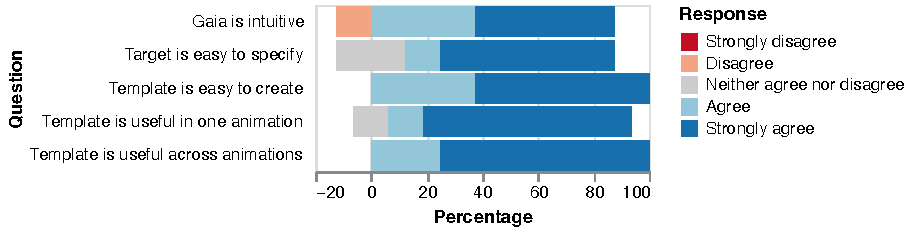
\includegraphics[width=\linewidth]{figs/user_ratings.pdf}
    \caption{User evaluations of primary features of \gaia{} using a 5-point Likert scale.}
%    \Description{User evaluations of primary features of \gaia{} using a 5-point Likert scale.}
    \label{fig:user_ratings.pdf}
\end{figure}

\autoref{fig:user_ratings.pdf} shows the results of the questionnaire.
The overall satisfaction of \gaia{} is high.
Most of the participants (7/8) think \gaia{} is intuitive and easy to use (average AVG=4.25, SD=1.04, 1 means strongly disagree and 5 means strongly agree).
P8, who gave a rank of 2, said, "\textit{I couldn't understand the stagger at first, so I got stuck.}"
However, he reported that after understanding these basic concepts, writing \gaia{} became easier.
For the target selection, most participants (6/8) took a positive attitude (AVG=4.28, SD=0.92).
The template, one of the most important features of \gaia{}, is considered to be easy to create (AVG=4.63, SD=0.52), and proves beneficial for crafting individual animated infographics (AVG=4.63, SD=0.74) as well as multiple animated infographics (AVG=4.75, SD=0.46).

In the interview, all participants agreed that \gaia{} is an easy-to-use and powerful tool for creating animated infographics.
"\textit{It let me pay more effort on design instead of effect implementation.}" P5 commented.
Participants thought that certain key features, like target selection and templates, would not incur additional learning costs.
"\textit{People who have used D3 or DOM APIs can easily get started (specifying target)}" (P1). 
Besides, some participants think the target model helps simplify the creation.
P6 told us: "\textit{target selection is a list of elements, which is more clear compared to the DOM tree.}"
Some participants mentioned that the logic of creating and using templates is similar to functions (P2, P3, P5), and the parameters can be set intuitively (P6, P7).
As for the benefits of the template, most of the participants agreed that it saves time and facilitates exploration.
P4 said, "\textit{It (template) avoids to adjust elements one by one when animations are similar but different in target/duration}".
"\textit{It is also helpful when we need to modify the animation since we only need to change the template}" (P3).

We paid attention to the mistakes participants made during the task, and tried to analyze the causes.
Setting the wrong parameters or using the wrong template are the most common mistakes.
For example, P5 tried to set the \code{from} parameters to \code{Fade} in Task 1.
\gaia{} compiler ignored the wrong parameters without any warning, causing him to start doubting whether the code had compiled successfully.
This problem was also mentioned by P1 and P7. "\textit{The system will not highlight the modified. Sometimes I wonder if the changes have taken effect}" (P1).
In addition, we also noticed that the wiping direction of the bars and lines in Task 4 is easily overlooked.
After our hints, participants still had to switch and watch the video several times before they realized the difference.

We also asked about the disappointments and improvements for \gaia{}.
More than half of the participants (P1, P2, P3, P5, P7) mentioned the lack of links between specs, SVG, and target models is a pity.
This made the debugging difficult.
"\textit{It is tedious to find useful resources in different tabs. Develop an IDE for \gaia{} might be cool}" (P3).
Besides, P3 and P6 suggested that if lambda expressions can be used to compute some values (like duration or stagger), it will be more flexible.
Three participants (P2, P3, P6) mentioned there is no gallery or document to support exploration, which is useful for novices.


\subsection{Expert Interview}
\label{ssec:expert_interview}

\gaia{} has already been used in real-world practices by several experts in the domain of animation creation and visualization. 
We kept in contact with these experts and collected their feedback during the development of \gaia{}.
In this section, we interviewed three of them (denoted as E1-3) in a semi-structured way to gather their perspectives from different views (creators and designers).
E1 has participated in some projects related to animation creation and has expertise in animation design. 
E2 is a researcher in visualization and data analysis, having experience with animation creation for more than 3 years.
The research direction of E3 is data storytelling. She has experience using animation creation tools for more than 6 years.

\subsubsection{Existing and Potential Usage Scenarios}

E1 used \gaia{}, from the view of a creator, to create videos for two months up to the time of the interview.
Both E2 and E3 use \gaia{} as the underlying animation engine to complete research work on interactive authoring and automatic generation of data videos.
They used \gaia{} for two years and one year, respectively, gaining insights into its functionality from the perspectives of creators and designers.
The work on E2 is being delivered, and the work of E3 has been published in the top conferences of visualization.
All of them think \gaia{} reduces the complexity of their tasks, simplifying the workflow and avoiding code-level implementation of motion effects.
E1 said, "\textit{\gaia{} is more powerful and customizable than other tools like PPT and can be easily integrated into our project, linking other code to the animation engine}".
E2 and E3 tried to use \gaia{} as an abstraction layer for incorporating large language models (LLMs) into the process of generating data videos.
"\textit{The most valuable aspect is that it is an abstraction layer to express, save, and reuse animations}", E2 told us.

When discussing the potential usage of \gaia{}, E1 commented that \gaia{} can support animation design in larger scenarios, not limited to 2D graphics (\eg SVG), such as VR and 3D.
Besides, E1 mentioned that \gaia{} can contribute to the adaptive UI design, such as the transition between two UI layouts.
Both E2 and E3 think that \gaia{} can benefit a wide range of users, including researchers, designers and data scientists.
"\textit{As a researcher on storytelling, I am one of the beneficiaries. In addition, \gaia{} can also help popular science video producers save time}", E3 said.

\subsubsection{Expressiveness and Learning Curve}

All of them agree that \gaia{} spec is simple and well structured, having a good balance between expressiveness and conciseness.
"\textit{All animations I need can be done via changing the parameters of templates}", E3 said.
The JSON grammar and CSS selectors make \gaia{} easy to learn and use, especially for users with a programming background (E1).
"\textit{The animations I designed are usually complex. \gaia{}'s grammar offers a controllable and predictable way to specify them.}", E1 said.
Compared to other tools like D3 and animated Vega-Lite, both E2 and E3 think \gaia{} targets a different problem and is more suitable for creating animated infographics, as other tools focus on transition and interaction, or employ a data-driven approach.

However, E1 pointed out that it is difficult for \gaia{} to express some relatively small animations, such as the blinking effect of a cat.
\textit{"My project manager thinks a large movement or stagger of multiple elements is more difficult to achieve than a small effect. But (in \gaia{}) the opposite is true" (E1)}.
E2 mentioned that when integrating \gaia{} into an automatic workflow, the parameters make things difficult.
"\textit{Some highly stylized or unusual animations are difficult to create in \gaia{}}", said E3, "\textit{they might require familiarity with \gaia{} or implementation through code.}"
Overall, though, all agreed that the ratio between the capabilities offered by \gaia{} and the cost of learning was high.

For the learning curve of \gaia{}, E1 and E3 believe that users still need to understand the JSON format and some basic knowledge in visualization and animation creation, but after that, the curve becomes very flat. 
"I tried to explain my animation design to a project manager using \gaia{}, but I find it is difficult as they even don't know the JSON" (E1).
"\textit{The difficulty of getting started depends on other experience with similar specs and background knowledge}", E3 said, "\textit{but for a programmer, this is not a problem.}"
These insights are also consistent with what we observed in the user study. 
E2 told us, "\textit{it is much easier than D3, and has a similar learning curve to animated Vega-Lite.}"

\subsubsection{Template Usage}

\gaia{} is the first high-level grammar that supports the template and supplies reusing for animations.
E1 thought the template is like functions in programming languages and can be used to encapsulate animations.
"\textit{I use templates all the time}", E1 told us, "\textit{It allows me to manage animations more clearly, even sometimes I don't reuse them.}"
In the work of E2, some complex animations are encapsulated as templates with readable names describing the effect (\eg \code{Pie-wheel-in-and-legend-fly-in}).
Then providing these animation names, element information (obtained from the target model) and narrations as prompts, LLMs can generate animations automatically.
"\textit{LLMs can understand the meaning of the animation, combine the narrative with the appropriate animation for the elements without considering the implementation details}", says E2.
E3 said that as long as a template meets the needs, she will use it first.
"\textit{They are intuitive and save time}" (E3).


\subsubsection{Extensibility}

\gaia{} allows users to create templates and extend the library in a declarative way.
E2 and E3 collaborated for an extended period.
As designers, they all craft templates according to their own needs.
E2 mentioned, "\textit{Sometimes we share the templates we have created and leave the ones we might use in our projects.}"
E2 created more than 20 templates using high-level specs, but E3 doesn't think it is necessary to create so many templates.
"\textit{Templates are most commonly used animations. A few templates will cover the needs of most cases}" (E3).

As for the consideration when designing templates, E1 thought the key point was the complexity.
"\textit{I hope the template is sufficiently generic without being overly complex to comprehend, as this would be detrimental for both myself and my collaborators}" (E1).
E2 commented the design of templates should consider the style of animated elements.
He also pointed out that some settings in a template are more likely to be changed to fit different scenarios.
As an example, he mentioned that bars might enter quickly at the beginning in some cases, but slowly in others, so letting the duration of these key elements be customizable is a good idea.

E2 also provides some insights for \gaia{} improvements. He suggested implementing effects for specific purposes.
For example, the effects used to create animations for children need to be more fun (like bar bounce).
In addition, emotional factors may also be a consideration to expand the effects.
